\scanpage{32}
% @ 1–3
Si $A$ est l'algèbre \inserted{affine} d'un monoïde \inserted{affine $G$} sur $k$, [i.e. $A$ est muni, en plus de la comultiplication $\pi$ \inserted{\unsure{assoc.} et unitaire} d'une multiplication bilinéaire \inserted{ass. unitaire} \deleted{\unsure{qui en fait un}} qui est de plus \uline{commutative}, et $\pi$ est un
% @ 4–8
hom d'\unsure{algèbre|algèbres}] alors $\forall\,k'$, les \unsure{élmts|éléments} de \inserted{$V(A)(k')=$} $\mathrm{Hom}_{k\text{-mod.}}(A,k')$ \inserted{i.e. les hom \unsure{$k$-lin|linéaires} $A\to k'$} sont \unsure{appelés|appelées} les ``\uline{distributions} de $G$ à \deleted{\unsure{valeurs}} coeff dans $k'$'', notés $\mathrm{Dist}(G)(k')$\inserted{[algèbre des distributions]}. Donc \deleted{\unsure{on a}} elles forment une $k'$-algèbre [``l'algèbre du \deleted{groupe} \inserted{monoïde} \deleted{\unsure{G}} $G$ à coeff dans $k'$''] et on aura une inclusion de monoïdes
% @ 9
\[
 G\deleted{(k')}\hookrightarrow\mathrm{Dist}(G)(k')^{\unsure{\times|x}}
\]
% @ 10–11
et si $G$ est un groupe
\[
 G(k')\hookrightarrow\mathrm{Dist}(G)(k')^{*}
\]
\margin{[pratiquement jamais un isom]}

% @ 11 left margin
% margin note written sideways
\margin{\diagram{\rotatebox{90}{\begin{tikzcd}[ampersand replacement=\&,column sep=small,row sep=small,font=\scriptsize]
 \mathrm{Dist}(X) \arrow[r,"{\pi}"] \& \mathrm{Dist}(X)\times\mathrm{Dist}(X) \& \pi(x)={} \\
 \deleted{e} \arrow[r,phantom,"{\deleted{\to}}"] \& \deleted{\mathrm{Dist}(X)} \& \\
 e \arrow[uu] \& \&
\end{tikzcd}}}}

% @ 12–13
\figure{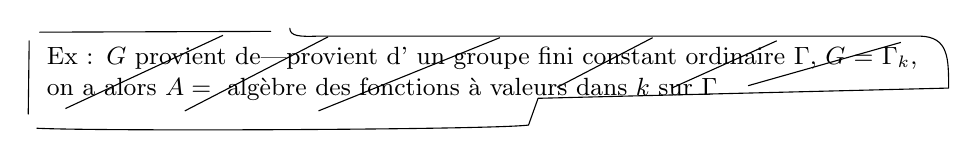
\begin{tikzpicture}[x=\linewidth,y=1cm]
\node[anchor=north west,inner sep=0pt,text width=.92\linewidth,font=\small] at (.025,.02)
 {\deleted{Ex : $G$ \inserted{\unsure{provient de|provient d'}} un groupe fini \deleted{constant} \inserted{ordinaire} $\Gamma$, $G=\Gamma_k$, on a alors $A={}$ algèbre des fonctions \inserted{à valeurs dans $k$} sur $\Gamma$}};
\draw[line cap=round,line join=round] (.018,.21) -- (.26,.22)
 (.28,.26) .. controls (.28,.16) and (.29,.15) .. (.31,.16)
 -- (.94,.16) .. controls (.97,.15) and (.97,-.12) .. (.97,-.50)
 -- (.54,-.63) -- (.53,-.97) .. controls (.49,-1.03) and (.08,-1.05) .. (.015,-1.01)
 (.006,-.83) -- (.007,.10);
\draw (.045,-.76)--(.21,.17) (.17,-.79)--(.32,.15)
 (.31,-.79)--(.50,.14) (.56,-.49)--(.66,.14)
 (.68,-.50)--(.79,.10) (.76,-.47)--(.92,.08);
\end{tikzpicture}}

% @ 14–17
\[
 gg^{-1}=1
\]
\diagram{\begin{tikzcd}[ampersand replacement=\&,column sep=large]
 G \arrow[dr,"{\unsure{\dot p|p|j}}"] \arrow[r,dash,"{\mathrm{id}_G\times\sigma}",to path={-- ++(1.6pt,0pt) -- ++(1.3pt,1.3pt) -- ++(-1.9pt,-2.4pt) -- ++(.7pt,1.1pt) -- (\tikztotarget) \tikztonodes -- ++(0pt,-1.1pt)}] \& G\times G \arrow[r,"{\pi}",dash,to path={-- (\tikztotarget) \tikztonodes -- ++(0pt,-1.3pt)}] \& G \\
 \& e \arrow[ur,"{\varepsilon}"] \&
\end{tikzcd}}
% @ 15 opposite first diagram
\[
 \deleted{A\to A\otimes A}
\]

% @ 18–21
\diagram{\begin{tikzcd}[ampersand replacement=\&,column sep=large]
 x\sigma y \& (x,y) \arrow[l,maps to] \& \\
 A \& A\otimes A \arrow[l] \& A \arrow[l,"{\pi}"] \arrow[dl,"{\varepsilon}"] \\
 \& k \arrow[ul,"p"] \&
\end{tikzcd}}
% @ 18–21 left margin
% margin note written sideways
\margin{\diagram{\rotatebox{90}{\begin{tikzcd}[ampersand replacement=\&,column sep=small,row sep=small,font=\scriptsize]
 \deleted{X\times Y}\;A \arrow[dr,"{\varepsilon}"'] \& A\otimes A \arrow[l] \arrow[d,shift left] \arrow[d,shift right] \& x\otimes y \\
 \& k \& \unsure{\varepsilon(x)\varepsilon(y)|\varepsilon x)\varepsilon y)}
\end{tikzcd}}}}
% archive sheet number: 31
